\documentclass{article}
\usepackage{amsfonts} % For \mathbb
\usepackage{amsmath} % For align*
\usepackage{enumitem} % For customisable list labels
\usepackage{graphicx} % For images
\usepackage{siunitx} % For units
\graphicspath{{./images/}}

\newcommand{\adj}{\operatorname{adj}}
\newcommand{\rank}{\operatorname{rank}}
\newcommand{\Span}{\operatorname{Span}}
\newenvironment{amatrix}[1]{%
  \left(\begin{array}{@{}*{#1}{c}|c@{}}
    }{%
  \end{array}\right)
}

\title{Advanced Engineering Mathematics Vectors, Matrices, and Vector Calculus by Dennis G. Zill Notes}
\author{Chris Doble}
\date{June 2023}

\begin{document}

\maketitle

\tableofcontents

\section{Vectors}

\subsection{Vectors in 2-Space}

\begin{itemize}
  \item The zero vector can be assigned any direction

  \item The vectors $\textbf{i}$ and $\textbf{j}$ are known as the \textbf{standard basis vectors} for $\mathbb{R}^2$
\end{itemize}

\subsection{Vectors in 3-Space}

\begin{itemize}
  \item In $\mathbb{R}^3$ the octant in which all coordinates are positive is known as the \textbf{first octant}. There is no agreement for naming the other seven octants.
\end{itemize}

\subsection{Dot Product}

\begin{itemize}
  \item The \textbf{dot product} is also known as the \textbf{inner product} or the \textbf{scalar product} and is denoted $\mathbf{a} \cdot \mathbf{b}$

  \item Two non-zero vectors are orthogonal iff their dot product is $0$

  \item The zero vector is considered orthogonal to all vectors

  \item The angles $\alpha$, $\beta$, and $\gamma$ between a vector and the unit vectors $\mathbf{i}$, $\mathbf{j}$, and $\mathbf{k}$, respectively are called the \textbf{direction angles} of the vector

  \item The cosines of a vectors direction angles (the \textbf{direction cosines}) can be calculated as

        \begin{align*}
          \cos \alpha & = \frac{\mathbf{a} \cdot \mathbf{i}}{||\mathbf{a}|| ||\mathbf{i}||} \\
                      & = \frac{a_1}{||\mathbf{a}||}                                        \\
          \cos \beta  & = \frac{\mathbf{a} \cdot \mathbf{j}}{||\mathbf{a}|| ||\mathbf{j}||} \\
                      & = \frac{a_2}{||\mathbf{a}||}                                        \\
          \cos \gamma & = \frac{\mathbf{a} \cdot \mathbf{k}}{||\mathbf{a}|| ||\mathbf{k}||} \\
                      & = \frac{a_3}{||\mathbf{a}||}
        \end{align*}

        Equivalently, these can be calculated as the components of the unit vector $\mathbf{a} / ||\mathbf{a}||$.

  \item To find the component of a vector $\mathbf{a}$ in the direction of a vector $\mathbf{b}$ \[\text{comp}_\mathbf{b} \mathbf{a} = ||\mathbf{a}|| \cos \theta = \frac{\mathbf{a} \cdot \mathbf{b}}{||\mathbf{b}||}\]

  \item To project a vector $\mathbf{a}$ onto a vector $\mathbf{b}$ \[\text{proj}_\mathbf{b} \mathbf{a} = (\text{comp}_\mathbf{b} \mathbf{a}) \frac{\mathbf{b}}{||\mathbf{b}||} = \left( \frac{\mathbf{a} \cdot \mathbf{b}}{\mathbf{b} \cdot \mathbf{b}} \right) \mathbf{b}\]
\end{itemize}

\subsection{Cross Product}

\begin{itemize}
  \item The cross product is only defined in $\mathbb{R}^3$

  \item The \textbf{scalar triple product} of vectors $\mathbf{a}$, $\mathbf{b}$, and $\mathbf{c}$ is defined as \[\mathbf{a} \cdot (\mathbf{b} \times \mathbf{c}) = (\mathbf{a} \times \mathbf{b}) \cdot \mathbf{c} = \begin{vmatrix}
            a_1 & a_2 & a_3 \\
            b_1 & b_2 & b_3 \\
            c_1 & c_2 & c_3
          \end{vmatrix}\]

  \item The area of a parallelogram with sides $\mathbf{a}$ and $\mathbf{b}$ is $||\mathbf{a} \times \mathbf{b}||$

  \item The area of a triangle with sides $\mathbf{a}$ and $\mathbf{b}$ is $\frac{1}{2} ||\mathbf{a} \times \mathbf{b}||$

  \item The volume of a paralleleipied with sides $\mathbf{a}$, $\mathbf{b}$, and $\mathbf{c}$ is $|\mathbf{a} \cdot (\mathbf{b} \times \mathbf{c})|$

  \item $\mathbf{a} \cdot (\mathbf{b} \times \mathbf{c}) = 0$ iff $\mathbf{a}$, $\mathbf{b}$, and $\mathbf{c}$ are coplanar
\end{itemize}

\subsection{Lines and Planes in 3-Space}

\begin{itemize}
  \item There is a unique line between any two points $\mathbf{r_1}$ and $\mathbf{r_2}$ in 3-space. The equation for that line is \[\mathbf{r} = \mathbf{r_1} + t (\mathbf{r_2} - \mathbf{r_1}) = \mathbf{r_1} + t \mathbf{a}\] where $t$ is called a \textbf{parameter}, the nonzero vector $\mathbf{a}$ is called a \textbf{direction vector}, and its components are called \textbf{direction numbers}.

  \item Equating the components of the equation above we find \begin{align*}
          x & = r_1 + t a_1  \\
          y & = r_2 + t a_2  \\
          z & = r_3 + t a_3.
        \end{align*} These are the \textbf{parametric equations} for the line through $\mathbf{r_1}$ and $\mathbf{r_2}$.

  \item By solving the parametric equations for $t$ and equating the results we find the \textbf{symmetric equations} for the line \[t = \frac{x - r_1}{a_1} = \frac{y - r_2}{a_2} = \frac{z - r_3}{a_3}.\]

  \item Given a point $P_1$ and a vector $\mathbf{n}$, there exists only one plane containing $P_1$ with $\mathbf{n}$ normal. The vector from $P_1$ to another point $P$ on that plane will be perpendicular to $\mathbf{n}$, so the equation for the plane is \[\mathbf{n} \cdot (\mathbf{r} - \mathbf{r}_1) = 0\] where $\mathbf{r} = \overrightarrow{O P}$ and $\mathbf{r_1} = \overrightarrow{O P_1}$. If \[\mathbf{n} = a \hat{\mathbf{i}} + b \hat{\mathbf{j}} + c \hat{\mathbf{k}}\] the cartesian form of this equation is \[a (x - x_1) + b (y - y_1) + c (z - z_1) = 0\] and is called the \textbf{point-normal form}.

  \item The graph of any equation $a x + b y + c z + d = 0$, where $a$, $b$, and $c$ are not all zero, is a plane with the normal vector $\mathbf{n} = a \hat{\mathbf{i}} + b \hat{\mathbf{j}} + c \hat{\mathbf{k}}$.

  \item Given three noncollinear points, a normal vector can be found by forming two vectors from two pairs of points and take their cross product.

  \item A line and a plane that aren't parellel intersect at a single point.

  \item Two planes that aren't parallel must intersect in a line.
\end{itemize}

\subsection{Vector Spaces}

\begin{itemize}
  \item The length of a vector is called its \textbf{norm}

  \item The process of multipying a vector by the reciprocal of its norm is called \textbf{normalizing} the vector

  \item Two nonzero vectors $\mathbf{a}$ and $\mathbf{b}$ in $\mathbb{R}^n$ are said to be orthogonal if $\mathbf{a} \cdot \mathbf{b} = 0$
\end{itemize}

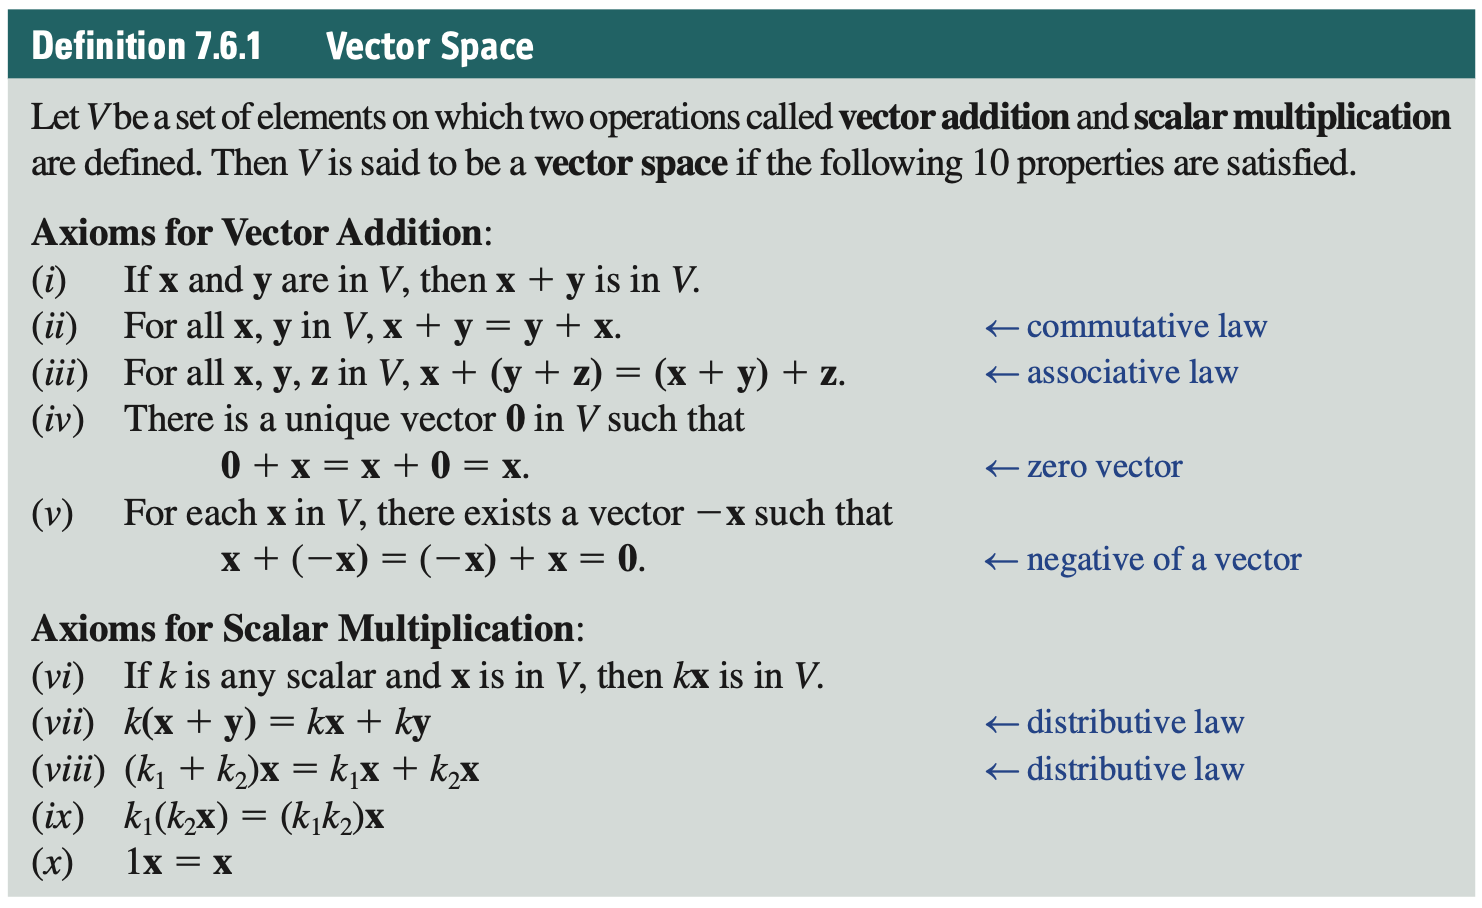
\includegraphics[scale=0.443]{vector-space}

\begin{itemize}
  \item If a subset $W$ of a vector space $V$ is itself a vector space under the operations of vector addition and scalar multiplication defined on $V$, then $W$ is called a \textbf{subspace} of $V$

  \item Every vector space has at least two subspaces: itself and the zero subspace $\{\mathbf{0}\}$

  \item A set of vectors $\{\mathbf{x_1}, \mathbf{x_2}, \ldots, \mathbf{x_n}\}$ is said to be \textbf{linearly independent} if the only constants satisfying the equation \[k_1 \mathbf{x_1} + k_2 \mathbf{x_2} + \cdots + k_n \mathbf{x_n} = \mathbf{0}\] are $k_1 = k_2 = \cdots = k_n = 0$. If the set of vectors is not linearly independent it is said to be \textbf{linearly dependent}.

  \item If a set of vectors $B = \{\mathbf{x}_1, \mathbf{x}_2, \ldots, \mathbf{x}_n\}$ in a vector space $V$ is linearly independent and every vector in $V$ can be expressed as a linear combination of vectors in $B$ then $B$ is said to be a \textbf{basis} for $V$.

  \item The number of vectors in a basis $B$ for a vector space $V$ is said to be the \textbf{dimension} of the space.

  \item If the basis of a vector space contains a finite number of vectors, then the space is \textbf{finite dimensional}; otherwise it is \textbf{infinite dimensional}.

  \item If $S$ denotes any set of vectors $\{\mathbf{x}_1, \mathbf{x}_2, \ldots, \mathbf{x}_n\}$ in a vector space $V$, then the set of all linear combinations of the vectors in $S$ \[c_1 \mathbf{x}_1 + c_2 \mathbf{x}_2 + \cdots + c_n \mathbf{x}_n\] is called the \textbf{span} of the vectors and is denoted $\Span(S)$.

  \item $\Span(S)$ is a subspace of $V$ and is said to be a subspace spanned by its vectors $\mathbf{x}_1, \mathbf{x}_2, \ldots, \mathbf{x}_n$.

  \item If $V = \Span(S)$ then $S$ is said to be a \textbf{spanning set} for the vector space $V$ or that $S$ \textbf{spans} $V$.
\end{itemize}

\subsection{Gram–Schmidt Orthogonalization Process}

\begin{itemize}
  \item An \textbf{orthonormal basis} is a basis whose vectors are mutually orthogonal and are unit vectors.

  \item If $B = \{\mathbf{w}_1, \mathbf{w}_2, \ldots, \mathbf{w}_n\}$ is an orthonormal basis for $\mathbb{R}^n$ then an arbitrary vector $\mathbf{u}$ can be expressed as \[\mathbf{u} = (\mathbf{u} \cdot \mathbf{w}_1) \mathbf{w}_1 + (\mathbf{u} \cdot \mathbf{w}_2) \mathbf{w}_2 + \cdots + (\mathbf{u} \cdot \mathbf{w}_n) \mathbf{w}_n\]

  \item The \textbf{Gram-Schmidt Orthogonalization Process} is a process for converting any basis of a vector space into an orthonormal basis. First the basis vectors are made orthogonal to each other, then they are normalized. More specifically, to convert a basis $B = \{\mathbf{u}_1, \mathbf{u}_2, \ldots, \mathbf{u}_n\}$ into an orthogonal basis $B' = \{\mathbf{v}_1, \mathbf{v}_2, \ldots, \mathbf{v}_n\}$

        \begin{enumerate}
          \item Let $\mathbf{v}_1 = \mathbf{u}_1$

          \item Let $\mathbf{v}_2 = \mathbf{u}_2 - \text{proj}_{\mathbf{v}_1} \mathbf{u}_2$

          \item \ldots

          \item Let $\mathbf{v}_n = \mathbf{u}_n - \text{proj}_{\mathbf{v}_1} \mathbf{u}_n - \text{proj}_{\mathbf{v}_2} \mathbf{u}_n - \cdots - \text{proj}_{\mathbf{v}_{n - 1}} \mathbf{u}_n$
        \end{enumerate}

        and to convert $B'$ into an orthonormal basis $B'' = \{\mathbf{w}_1, \mathbf{w}_2, \ldots, \mathbf{w}_n\}$, normalize each $\mathbf{v}_i$, $i = 1, 2, \ldots, n$.
\end{itemize}

\section{Matrices}

\subsection{Matrix Algebra}

\begin{itemize}
  \item Vectors can be written as horizontal or vertical arrays of numbers

  \item A \textbf{matrix} is any rectangular array of numbers or functions \[\begin{pmatrix}
            a_{11} & a_{12} & \cdots & a_{1n} \\
            a_{21} & a_{22} & \cdots & a_{2n} \\
            \vdots &        &        & \vdots \\
            a_{m1} & a_{m2} & \cdots & a_{mn}
          \end{pmatrix}\]

  \item The numbers or functions in the array are called the \textbf{elements} or \textbf{entries} of the matrix

  \item If a matrix has $m$ rows and $n$ columns we say that its \textbf{size} is $m$ by $n$ or $m \times n$

  \item An $n \times n$ matrix is called a \textbf{square} matrix of \textbf{order $n$}

  \item The entry in the $i$th row and the $j$th column of an $m \times n$ matrix $\mathbf{A}$ is written $a_{ij}$

  \item An $m \times 1$ matrix \[\begin{pmatrix}
            a_1    \\
            a_2    \\
            \vdots \\
            a_n
          \end{pmatrix}\] is called a \textbf{column vector}

  \item A $1 \times n$ matrix \[\begin{pmatrix}
            a_1 & a_2 & \cdots & a_n
          \end{pmatrix}\] is called a \textbf{row vector}
\end{itemize}

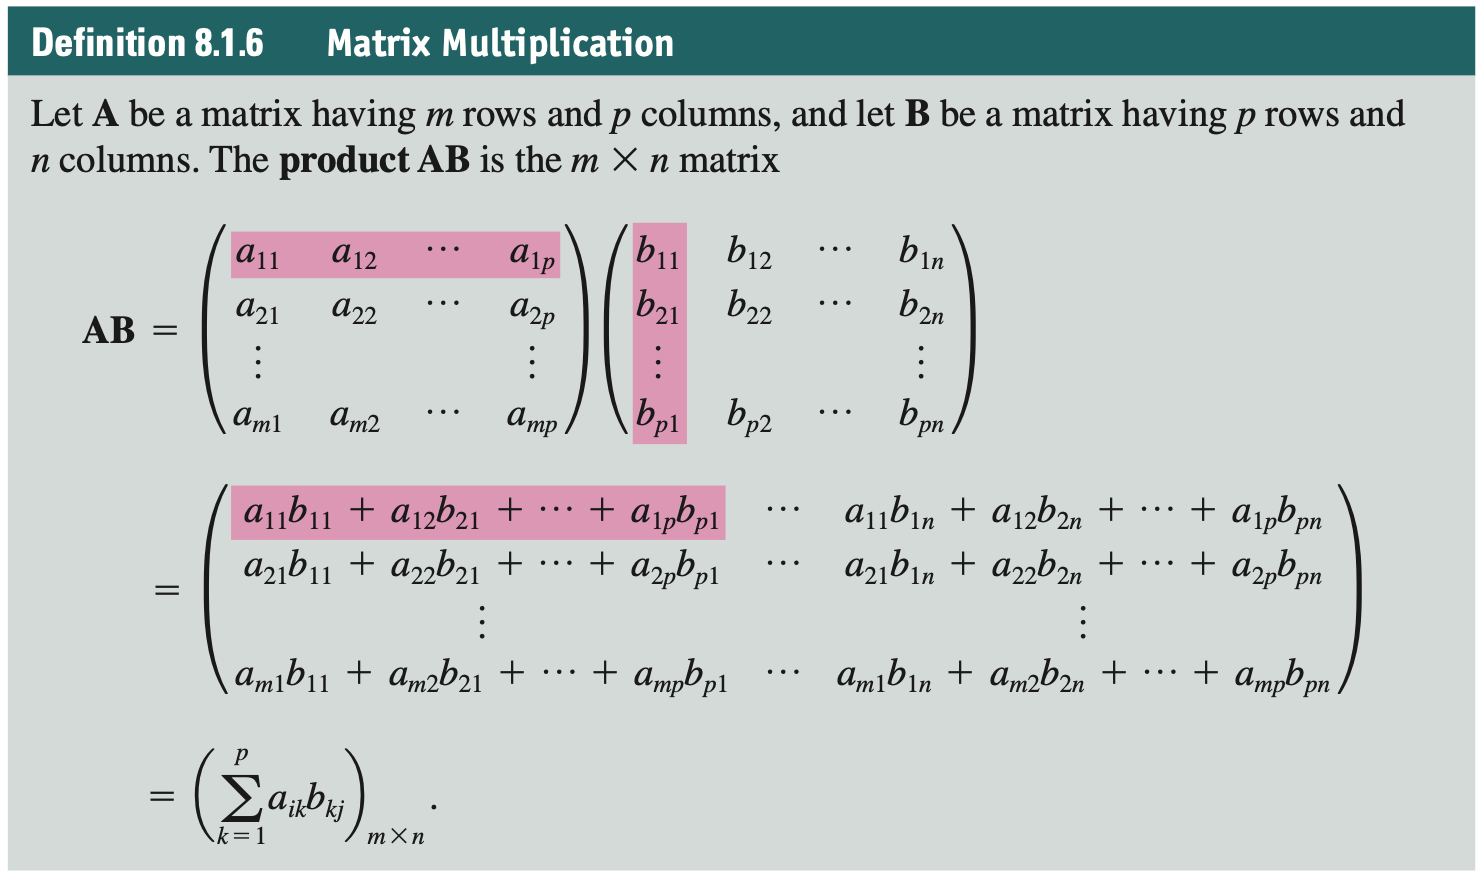
\includegraphics[scale=0.443]{matrix-multiplication}

\begin{itemize}
  \item Matrix multiplication is associative, i.e. $\mathbf{A} (\mathbf{B} \mathbf{C}) = (\mathbf{A} \mathbf{B}) \mathbf{C}$

  \item Matrix multiplication is distributive, i.e. $\mathbf{A} (\mathbf{B} + \mathbf{C}) = \mathbf{A} \mathbf{B} + \mathbf{A} \mathbf{C}$ and $(\mathbf{B} + \mathbf{C}) \mathbf{A} = \mathbf{B} \mathbf{A} + \mathbf{C} \mathbf{A}$

  \item The \textbf{transpose} of an $m \times n$ matrix $\mathbf{A}$ is an $n \times m$ matrix $\mathbf{A}^T$ \[\begin{pmatrix}
            a_{11} & a_{21} & \cdots & a_{m1} \\
            a_{12} & a_{22} & \cdots & a_{m2} \\
            \vdots &        &        & \vdots \\
            a_{1n} & a_{2n} & \cdots & a_{mn}
          \end{pmatrix}\] i.e. the matrix is flipped along the main diagonal
\end{itemize}

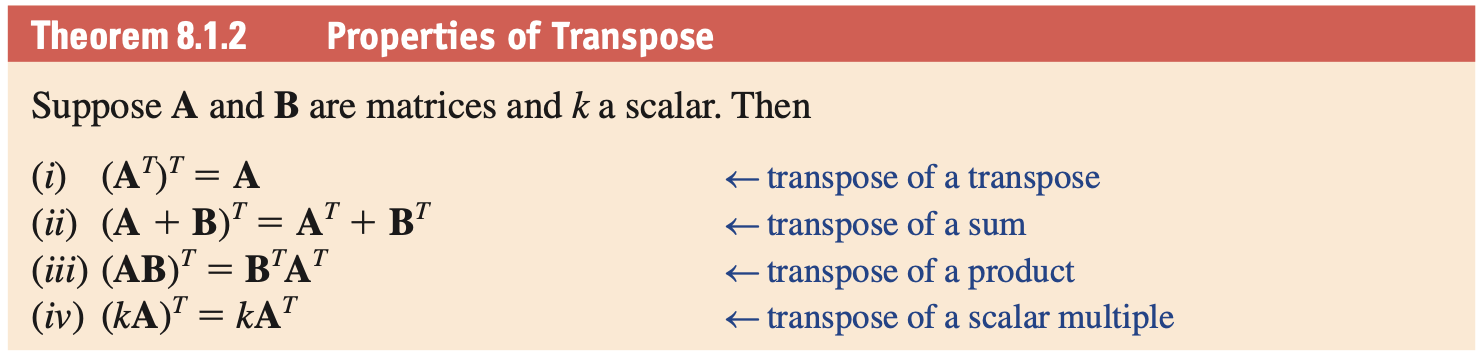
\includegraphics[scale=0.443]{transpose-properties}

\begin{itemize}
  \item A matrix that consists of all zero entries is called a \textbf{zero matrix}

  \item A square matrix is said to be a \textbf{triangular matrix} if all of its entries above or below the main diagonal are zeroes. More specifically they are called \textbf{lower triangular} and \textbf{upper triangular} matrices, respectively.

  \item A square matrix is called a \textbf{diagonal matrix} if all entries not on the main diagonal are 0.

  \item A square matrix whose entries on the main diagonal are all equal is called a \textbf{scalar matrix}

  \item A square matrix that has the property $\mathbf{A} = \mathbf{A}^T$ is called a \textbf{symmetric matrix}
\end{itemize}

\subsection{Systems of Linear Algebraic Equations}

\begin{itemize}
  \item In a linear system

        \begin{align*}
          a_{11} x_1 + a_{12} x_2 + \cdots + a_{1n} x_n & = b_1 \\
          a_{21} x_1 + a_{22} x_2 + \cdots + a_{2n} x_n & = b_2 \\
          \vdots                                                \\
          a_{m1} x_1 + a_{m2} x_2 + \cdots + a_{mn} x_n & = b_n \\
        \end{align*}

        the values $a_{ij}$ are called the \textbf{coefficients} and the values $b_n$ are called the \textbf{constants}

  \item If all the constants are zero the system is said to be \textbf{homogeneous}, otherwise it is \textbf{nonhomogeneous}

  \item A linear system is said to be \textbf{consistent} if it has at least one solution, otherwise it's \textbf{inconsistent}

  \item A linear system can be transformed into an equivalent system (i.e. one that has the same solutions) via three elementary operations:

        \begin{enumerate}
          \item Multiply an equation by a nonzero constant

          \item Interchange the positions of equations in the system

          \item Add a multiple of one equation to any other equation
        \end{enumerate}

  \item A linear system can be represented by an \textbf{augmented matrix}, e.g. \[\begin{amatrix}{2}
            a_{11} & a_{12} & b_1 \\
            a_{21} & a_{22} & b_2
          \end{amatrix}\]

  \item We say that two matrices are \textbf{row equivalent} if one can be obtained from the other via a series of elementary row operations

  \item \textbf{Gaussian elimination} is the process of applying elementary row operations to a matrix to put it into \textbf{row-echelon form} where:

        \begin{enumerate}
          \item The first nonzero entry in a row is a 1

          \item In subsequent rows, the first 1 entry appears to the right of the 1 entry in earlier rows

          \item Rows consisting of all zeroes are at the bottom of the matrix
        \end{enumerate}

  \item \textbf{Gauss-Jordan elimination} is the same as Gaussian elimination with an additional constraint that puts the matrix into \textbf{reduced row-echelon form} where a column containing a first entry 1 has zeroes everywhere else

  \item A homogeneous linear system always has a trivial solution where all variables are equal to zero and will have an infinite number of nontrivial solutions if the number of equations $m$ is less than the number of variables $n$, i.e. $m < n$

  \item If $\mathbf{X}_1$ is a solution to $\mathbf{A} \mathbf{X} = \mathbf{0}$, then so is $c \mathbf{X}_1$ for any constant $c$

  \item If $\mathbf{X}_1$ and $\mathbf{X}_2$ are solutions of $\mathbf{A} \mathbf{X} = \mathbf{0}$, then so is $\mathbf{X}_1 + \mathbf{X}_2$

  \item If a linear system contains more equations than variables it is said to be \textbf{overdetermined}; if it contains fewer equations than variables it is said to be \textbf{underdetermined}
\end{itemize}

\subsection{Rank of a Matrix}

\begin{itemize}
  \item The \textbf{rank} of a matrix $\mathbf{A}$ denoted $\rank(\mathbf{A})$ is the number of linearly independent row vectors in $\mathbf{A}$

  \item The row vectors of an $m \times n$ matrix $\mathbf{A}$ span a subspace of $\mathbb{R}^n$. This is called the \textbf{row space} of $\mathbf{A}$. The set of linearly independent row vectors in $\mathbf{A}$ are a basis for that subspace
\end{itemize}

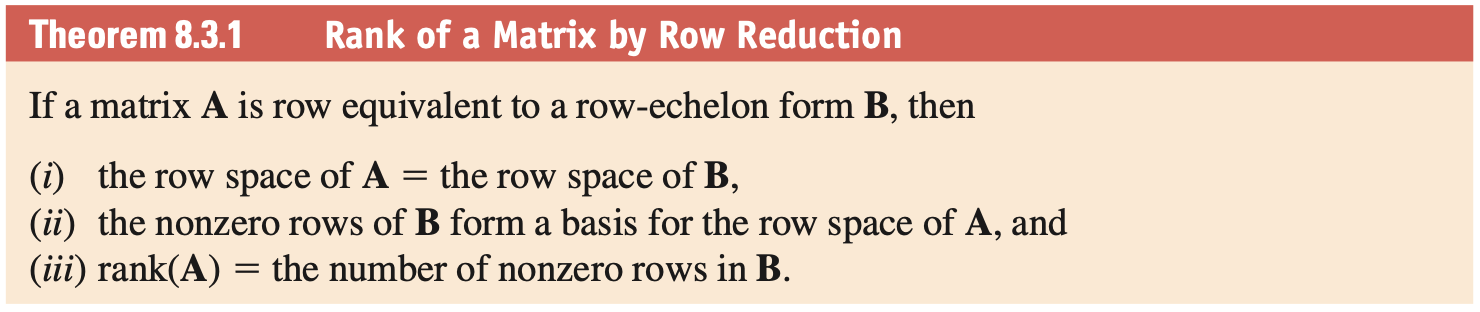
\includegraphics[scale=0.443]{rank-by-row-reduction}

\begin{itemize}
  \item A linear system of equations $\mathbf{A} \mathbf{X} = \mathbf{B}$ is consistent iff the rank of the coefficient matrix $\mathbf{A}$ is equal to the rank of the augmented matrix of the system $(\mathbf{A} | \mathbf{B})$

  \item Suppose a linear system $\mathbf{A} \mathbf{X} = \mathbf{B}$ with $m$ equations and $n$ variables is consistent. If $\rank(\mathbf{A}) = r$ then the solution of the system contains $n - r$ variables
\end{itemize}

\subsection{Determinants}

\begin{itemize}
  \item Suppose $\mathbf{A}$ is an $n \times n$ matrix. Associated with $\mathbf{A}$ is a number called the \textbf{determinant of $\mathbf{A}$} and is denoted by \[\det \mathbf{A} = \begin{vmatrix}
            a_{11} & a_{12} & \cdots & a_{1n} \\
            a_{21} & a_{22} & \cdots & a_{2n} \\
            \vdots &        &        & \vdots \\
            a_{n1} & a_{n2} & \cdots & a_{nn}
          \end{vmatrix}\]

  \item A determinant of an $n \times n$ matrix is called a \textbf{determinant of order $n$}

  \item The determinant of a $1 \times 1$ matrix is the element of the matrix

  \item Each element in an $n \times n$ matrix has an associated \textbf{cofactor} defined as \[a_{ij} = (-1)^{i + j} M_{ij}\] where $M_{ij}$ is the determinant of the $(n - 1) \times (n - 1)$ matrix produced by deleting row $i$ and column $j$ from $\mathbf{A}$

  \item The determinant of an arbitrary $n \times n$ matrix $\mathbf{A}$ can be calculated by choosing an arbitrary row or column and summing the products of each element in that column/row with their cofactors, e.g. if we choose the first row of a $3 \times 3$ matrix then

        \begin{align*}
          \begin{vmatrix}
            a_{11} & a_{12} & a_{13} \\
            a_{21} & a_{22} & a_{23} \\
            a_{31} & a_{32} & a_{33}
          \end{vmatrix} & = a_{11} M_{11} + a_{12} M_{12} + a_{13} M_{13}                                                        \\
                                      & = a_{11} \begin{vmatrix}
                                                   a_{22} & a_{23} \\
                                                   a_{32} & a_{33}
                                                 \end{vmatrix} - a_{12} \begin{vmatrix}
                                                                          a_{21} & a_{23} \\
                                                                          a_{31} & a_{33}
                                                                        \end{vmatrix} + a_{13} \begin{vmatrix}
                                                                                                 a_{21} & a_{22} \\
                                                                                                 a_{31} & a_{32}
                                                                                               \end{vmatrix}                   \\
                                      & = a_{11} (a_{22} |a_{33}| - a_{23} |a_{32}|) - a_{12} (a_{21} |a_{33} - a_{23} |a_{31}|) \\
                                      & \qquad + a_{13} (a_{21} |a_{32}| - a_{22} |a_{31}|)
        \end{align*}
\end{itemize}

\subsection{Properties of Determinants}

\begin{itemize}
  \item The determinant of a matrix and its transpose are the same

  \item If any two rows/columns of a matrix are the same its determinant is zero

  \item If all the entries in a row/column of a matrix are zero, then its determinant is zero

  \item Interchanging any two rows/columns of a matrix negates its determinant

  \item Multiplying a row/column of a matrix by a nonzero real number $k$ also multiplies the determinant by $k$

  \item If $\mathbf{A}$ and $\mathbf{B}$ are both $n \times n$ matrices, then $\det \mathbf{A} \mathbf{B} = \det \mathbf{A} \cdot \det \mathbf{B}$

  \item Adding a multiply of one row/column to another doesn't change the determinant

  \item The determinant of a triangular matrix is the product of the entries along the main diagonal

  \item Sometimes it's faster to calculate a matrix's determinant by reducing it to row-echelon form and multiplying the elements along the main diagonal than performing cofactor expansion

  \item Multiplying the entries of a row/column with the cofactors of another row/colum and summing the results always equals zero
\end{itemize}

\subsection{Inverse of a Matrix}

\begin{itemize}
  \item Given an $n \times n$ matrix $\mathbf{A}$, if there exists another $n \times n$ matrix $\mathbf{B}$ such that $\mathbf{A} \mathbf{B} = \mathbf{B} \mathbf{A} = \mathbf{I}$ then $\mathbf{A}$ is said to be \textbf{nonsingular} or \textbf{invertible} and $\mathbf{B}$ is said to be the unique \textbf{inverse} of $\mathbf{A}$, i.e. $\mathbf{B} = \mathbf{A}^{-1}$

  \item Some $n \times n$ matrices don't have an inverse and are called \textbf{singular}

  \item The \textbf{adjoint} of an $n \times n$ matrix $\mathbf{A}$ is the transpose of the matrix of cofactors corresponding to the entries of $\mathbf{A}$ \[\adj \mathbf{A} = \begin{pmatrix}
            C_{11} & C_{12} & \ldots & C_{1n} \\
            C_{21} & C_{22} & \ldots & C_{2n} \\
            \vdots &        &        & \vdots \\
            C_{n1} & C_{n2} & \ldots & C_{nn}
          \end{pmatrix}^T = \begin{pmatrix}
            C_{11} & C_{21} & \ldots & C_{n1} \\
            C_{12} & C_{22} & \ldots & C_{n2} \\
            \vdots &        &        & \vdots \\
            C_{1n} & C_{2n} & \cdots & C_{nn}
          \end{pmatrix}\]

  \item If $\mathbf{A}$ is an $n \times n$ matrix and $\det \mathbf{A} \ne 0$ then \[\mathbf{A}^{-1} = \left( \frac{1}{\det \mathbf{A}} \right) \adj \mathbf{A}\]

  \item From the above, the inverse of a $2 \times 2$ matrix $\mathbf{A}$ is \[\mathbf{A}^{-1} = \frac{1}{\det \mathbf{A}} \begin{pmatrix}
            a_{22}  & -a_{12} \\
            -a_{21} & a_{11}
          \end{pmatrix}\]

  \item An $n \times n$ matrix $\mathbf{A}$ is nonsingular (has an inverse) if $\det \mathbf{A} \ne 0$
\end{itemize}

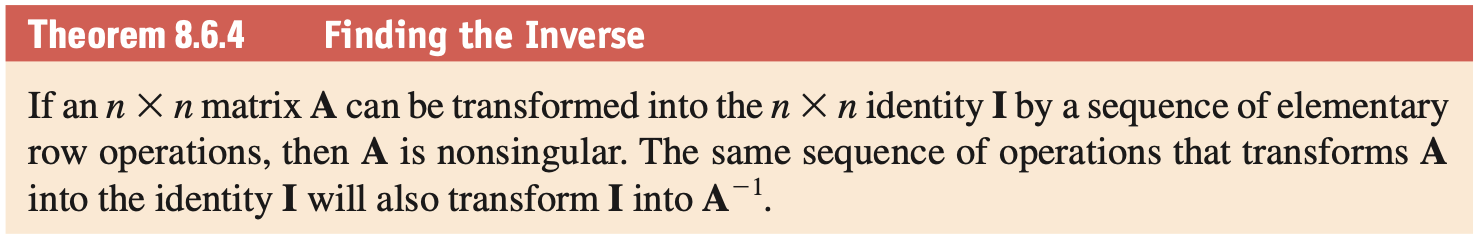
\includegraphics[scale=0.443]{row-operations-inverse}

\begin{itemize}
  \item Inverse matrices can be used to solve linear systems. If $\mathbf{A} \mathbf{X} = \mathbf{B}$ and $\mathbf{A}$ is invertible, then \[\mathbf{A}^{-1} \mathbf{A} \mathbf{X} = \mathbf{A}^{-1} \mathbf{B} \Rightarrow \mathbf{X} = \mathbf{A}^{-1} \mathbf{B}\]

  \item When $\det \mathbf{A} \ne 0$ the solution of the system $\mathbf{A} \mathbf{X} = \mathbf{B}$ is unique

  \item A homogeneous system of linear equations $\mathbf{A} \mathbf{X} = \mathbf{0}$ has only the trivial solution iff $\mathbf{A}$ is nonsingular and an infinite number of solutions iff it is singular
\end{itemize}

\subsection{Cramer’s Rule}

\begin{itemize}
  \item If $\mathbf{A}$ is the coefficient matrix of a linear system and $\det \mathbf{A} \ne 0$, then the solution of the system is given by

        \begin{align*}
          x_1 & = \frac{\det \mathbf{A}_1}{\det \mathbf{A}} \\
          x_2 & = \frac{\det \mathbf{A}_2}{\det \mathbf{A}} \\
          \vdots                                            \\
          x_n & = \frac{\det \mathbf{A}_n}{\det \mathbf{A}}
        \end{align*}

        where $\mathbf{A}_n$ is the matrix obtained by replacing column $n$ of $\mathbf{A}$ with the constants of the system.
\end{itemize}

\subsection{The Eigenvalue Problem}

\begin{itemize}
  \item If $\mathbf{A}$ is an $n \times n$ matrix, a number $\lambda$ is said to be an \textbf{eigenvalue} of $\mathbf{A}$ if there exists a nonzero solution vector $\mathbf{K}$ of the linear system $\mathbf{A} \mathbf{K} = \lambda \mathbf{K}$. The solution vector $\mathbf{K}$ is said to be an \textbf{eigenvector} corresponding to the eigenvalue $\lambda$.

  \item Rearranging the equation above we find \[(\mathbf{A} - \lambda \mathbf{I}) \mathbf{K} = \mathbf{0}\] which only has nontrivial solutions if $\det (\mathbf{A} - \lambda \mathbf{I}) = 0$.

  \item Calculating $\det (\mathbf{A} - \lambda \mathbf{I})$ results in an $n$-th degree polynomial in $\lambda$ called the \textbf{characteristic equation} of $\mathbf{A}$, the solutions to which are its eigenvalues.

  \item The eigenvector associated with a particular eigenvalue can be found by applying Gauss-Jordan elimination to the augmented matrix $(\mathbf{A} - \lambda \mathbf{I} | \mathbf{0})$.

  \item A nonzero constant multiple of an eigenvector is another eigenvector.

  \item If $\lambda$ is a complex eigenvalue of a matrix, then its conjugate $\lambda*$ is also an eigenvalue. If $\mathbf{K}$ is an eigenvector corresponding to $\lambda$ then its conjugate $\mathbf{K}*$ is an eigenvector corresponding to $\lambda*$.

  \item $\lambda = 0$ is an eigenvalue of a matrix iff the matrix isn't invertible

  \item The determinant of a matrix is the product of its eigenvalues

  \item If $\lambda$ is an eigenvalue of a matrix $\mathbf{A}$ with eigenvector $\mathbf{K}$, then $1 / \lambda$ is an eigenvalue of $\mathbf{A}^{-1}$ with the same eigenvector.

  \item The eigenvalues of a triangular matrix are the entries along the main diagonal.
\end{itemize}

\subsection{Powers of Matrices}

\begin{itemize}
  \item Any $n \times n$ matrix $\mathbf{A}$ satisfies its own characteristic equation, i.e. $\lambda$ can be replaced with $\mathbf{A}$ in the characteristic equation.

  \item This gives us an expression for $\mathbf{A}^n$ as a linear combination \[\mathbf{A}^n = c_0 \mathbf{I} + c_1 \mathbf{A} + c_2 \mathbf{A}^2 + \cdots + c_{n - 1} \mathbf{A}^{n - 1}.\] If we multiply this expression by $\mathbf{A}$ we get an expression for $\mathbf{A}^{n + 1}$ and we can replace the $\mathbf{A}^n$ term with the original expression. This can be repeated an arbitrary number of times to find expressions for any power of $\mathbf{A}$.

  \item The constants of the linear combination can be determined by substituting the matrix's eigenvalues into the characteristic equation, resulting in a linear system where the constants are the variables. Solving the system determines the constants.

  \item If $\mathbf{A}$ is a nonsingular matrix, the fact that it satisfies its own characteristic equation can be used to determine its inverse. This can be achieved by replacing $\lambda$ with $\mathbf{A}$ in its characteristic equation, solving for $\mathbf{I}$, and multiplying both sides by $\mathbf{A}^{-1}$. This results in an expression for $\mathbf{A}^{-1}$ as a linear combination of powers of $\mathbf{A}$.
\end{itemize}

\subsection{Orthogonal Matrices}

\begin{itemize}
  \item If $\mathbf{A}$ is a symmetric matrix with real entries, then the eigenvalues of $\mathbf{A}$ are real.

  \item If $\mathbf{A}$ is a symmetric matrix, then the eigenvectors corresponding to different eigenvalues are orthogonal.

  \item An $n \times n$ nonsingular matrix $\mathbf{A}$ is \textbf{orthogonal} if $\mathbf{A}^{-1} = \mathbf{A}^T$.

  \item An $n \times n$ matrix $\mathbf{A}$ is orthogonal iff its columns form an orthonormal set.

  \item If an $n \times n$ matrix $\mathbf{A}$ has $n$ distinct eigenvalues, an orthogonal matrix can be formed by normalizing its eigenvectors and using them as column vectors in a new matrix.
\end{itemize}

\subsection{Approximation of Eigenvalues}

\begin{itemize}
  \item Let $\lambda_1, \lambda_2, \ldots, \lambda_n$ denote the eigenvalues of an $n \times n$ matrix $\mathbf{A}$. The eigenvalue $\lambda_k$ is said to be the \textbf{dominant eigenvalue} of $\mathbf{A}$ if \[|\lambda_k| > |\lambda_i|, i = 1, 2, \ldots, n, i \ne k.\] An eigenvector corresponding to $\lambda_k$ is called the \textbf{dominant eigenvector} of $\mathbf{A}$.

  \item \textbf{Power iteration} is a method for approximating the dominant eigenvector of an $n \times n$ matrix $\mathbf{A}$.

        \begin{enumerate}
          \item Choose an arbitrary starting vector $\mathbf{X}_0$

          \item An approximation of the dominant eigenvector is $\mathbf{X}_m = \mathbf{A}^m \mathbf{X}_0$

          \item An approximation of the dominant eigenvalue is \[\lambda \approx \frac{\mathbf{A} \mathbf{X}_m \cdot \mathbf{X}_m}{\mathbf{X}_m \cdot \mathbf{X}_m}\]
        \end{enumerate}

  \item If $\mathbf{X}_m$ is computed via repeated multiplications of $\mathbf{A}$ rather than computing $\mathbf{A}^m$ in advance the entries of the intermediary vectors can become quite large and pose problems for computers. This can be avoided by normalising or scaling down the vectors after each iteration.

  \item The \textbf{method of deflation} is a way to find nondominant eigenvalues of an $n \times n$ symmetric matrix $\mathbf{A}$ that has eigenvalues \\ $|\lambda_1| > |\lambda_2| > |\lambda_3| \ge \cdots \ge |\lambda_n|$.

        \begin{enumerate}
          \item Compute the dominant eigenvalue $\lambda_1$ and normalised eigenvector $\mathbf{K}_1$ of the matrix using power iteration.

          \item Compute the matrix $\mathbf{B} = \mathbf{A} - \lambda_1 \mathbf{K}_1 \mathbf{K}_1^T$ which has eigenvalues \\ $0, \lambda_2, \lambda_3, \cdots, \lambda_n$

          \item Apply power iteration to find $\lambda_2$ and $\mathbf{K}_2$

          \item Repeat steps 2 and 3 to compute subsequent eigenvalues
        \end{enumerate}

  \item The \textbf{inverse power method} is a way to find the eigenvalue with smallest absolute value. If $\mathbf{A}$ is nonsingular then the eigenvalues of $\mathbf{A}^{-1}$ are the reciprocals of the eigenvalues of $\mathbf{A}$. This means the eigenvalue of $\mathbf{A}$ with smallest absolute value is the dominant eigenvalue of $\mathbf{A}^{-1}$ and can be found via power iteration.
\end{itemize}

\subsection{Diagonalization}

\begin{itemize}
  \item If an $n \times n$ nonsingular matrix $\mathbf{P}$ can be found so that $\mathbf{P}^{-1} \mathbf{A} \mathbf{P} = \mathbf{D}$ is a diagonal matrix, then we say that the $n \times n$ matrix $\mathbf{A}$ can be \textbf{diagonalised}, or is \textbf{diagonalisable}, and that \textbf{$\mathbf{P}$ diagonalises $\mathbf{A}$}.

  \item An $n \times n$ matrix $\mathbf{A}$ is diagonalisable iff $\mathbf{A}$ has $n$ linearly independent eigenvectors $\mathbf{K}_1, \mathbf{K}_2, \ldots, \mathbf{K}_n$. If we let $\mathbf{P} = \begin{pmatrix}
            \mathbf{K}_1 & \mathbf{K}_2 & \cdots & \mathbf{K}_n
          \end{pmatrix}$ then

        \begin{align*}
          \mathbf{A P} & = \begin{pmatrix}
                             \mathbf{A K_1} & \mathbf{A K_2} & \cdots & \mathbf{A K_n}
                           \end{pmatrix}                         \\
                       & = \begin{pmatrix}
                             \lambda_1 \mathbf{K}_1 & \lambda_2 \mathbf{K}_2 & \cdots & \lambda_n \mathbf{K}_n
                           \end{pmatrix} \\
                       & = \begin{pmatrix}
                             \mathbf{K}_1 & \mathbf{K}_2 & \cdots & \mathbf{K}_n
                           \end{pmatrix} \begin{pmatrix}
                                           \lambda_1 & 0         & \cdots & 0         \\
                                           0         & \lambda_2 & \cdots & 0         \\
                                           \vdots    &           & \ddots & \vdots    \\
                                           0         & 0         & \cdots & \lambda_n
                                         \end{pmatrix}                          \\
                       & = \mathbf{P} \mathbf{D}
        \end{align*}

  \item If an $n \times n$ matrix $\mathbf{A}$ has $n$ distinct eigenvalues, it is diagonalisable. If it has fewer than $n$ distinct eigenvalues it may still be diagonalisable.

  \item Symmetric matrices with real entries are always diagonalisable.
\end{itemize}

\subsection{LU-Factorisation}

\begin{itemize}
  \item If an $n \times n$ matrix $\mathbf{A}$ can be written as a product $\mathbf{A = L U}$ where $\mathbf{L}$ and $\mathbf{U}$ are lower and upper triangular matrices, respectively, then we say that $\mathbf{A = L U}$ is an \textbf{LU-factorisation} of $\mathbf{A}$.

  \item An $n \times n$ matrix $\mathbf{A}$ can have several LU-factorisations

  \item \textbf{Doolittle's method} is a method of performing LU-factorisation.

        \begin{enumerate}
          \item Assume the diagonal entries of $\mathbf{L}$ are $1$, i.e. $l_{ii} = 1, i = 1, 2, \ldots, n$

          \item Multiply $\mathbf{L}$ and $\mathbf{U}$ (with placeholder entries)

          \item Equate the resulting entries with those of the original matrix — this gives $n^2$ equations, but each equation only uses variables determined in previous equations allowing the system to be solved
        \end{enumerate}

  \item An alternative algorithm for Doolittle's method is

        \begin{enumerate}
          \item Perform elementary row operations on $\mathbf{A}$ until you have an upper triangular matrix $\mathbf{U}$

          \item Each time you add a $c$ times row $i$ to row $j$, record the $-c$ in the $j$-th row and $i$-th column of an identity matrix

          \item The matrix from step 2 is $\mathbf{L}$
        \end{enumerate}

  \item Given a linear system $\mathbf{A X = B}$, if $\mathbf{A}$ has an LU-factorisation the system can be solved as follows:

        \begin{enumerate}
          \item Rewrite the system $\mathbf{L U X} = B$

          \item Let $\mathbf{U X = Y}$ where \[\mathbf{Y} = \begin{pmatrix}
                    y_1    \\
                    y_2    \\
                    \vdots \\
                    y_n
                  \end{pmatrix}\]

          \item Solve $\mathbf{L Y = B}$ via forward substitution, i.e. find $y_1$, use that to find $y_2$, etc.

          \item Substitute the values of $y_n$ into $\mathbf{U X = Y}$ and solve via back substitution, i.e. find $x_n$, use that to find $x_{n - 1}$, etc.
        \end{enumerate}

  \item If a matrix $\mathbf{A}$ has an LU-factorisation $\mathbf{A = L U}$ then the determinant of $\mathbf{A}$ can be calculated as $\det \mathbf{A} = \det \mathbf{L} \cdot \det \mathbf{L}$ which is simply the product of the diagonal entries of $\mathbf{L}$ and $\mathbf{U}$

  \item If row interchanges are required to arrive at $\mathbf{U}$ then an LU-factorisation doesn't exist
\end{itemize}

\subsection{Cryptography}

\begin{itemize}
  \item If you define a mapping between a set of characters allowed in messages and a list of integers, messages can be represented as an $n \times m$ matrix, a nonsingular $n \times n$ matrix $\mathbf{A}$ can be used as an encryption key, and its inverse $\mathbf{A}^{-1}$ can be used as a decryption key.
\end{itemize}

\end{document}